\documentclass{exam}

\usepackage[scale=0.9]{geometry}
\usepackage[utf8]{inputenc}
\usepackage[french,english]{babel}
\usepackage[T1]{fontenc}
\usepackage{fontawesome}
\usepackage{enumitem}
\usepackage{graphicx}
\usepackage{amsmath}

\begin{document}

\begin{figure}
    \centering
    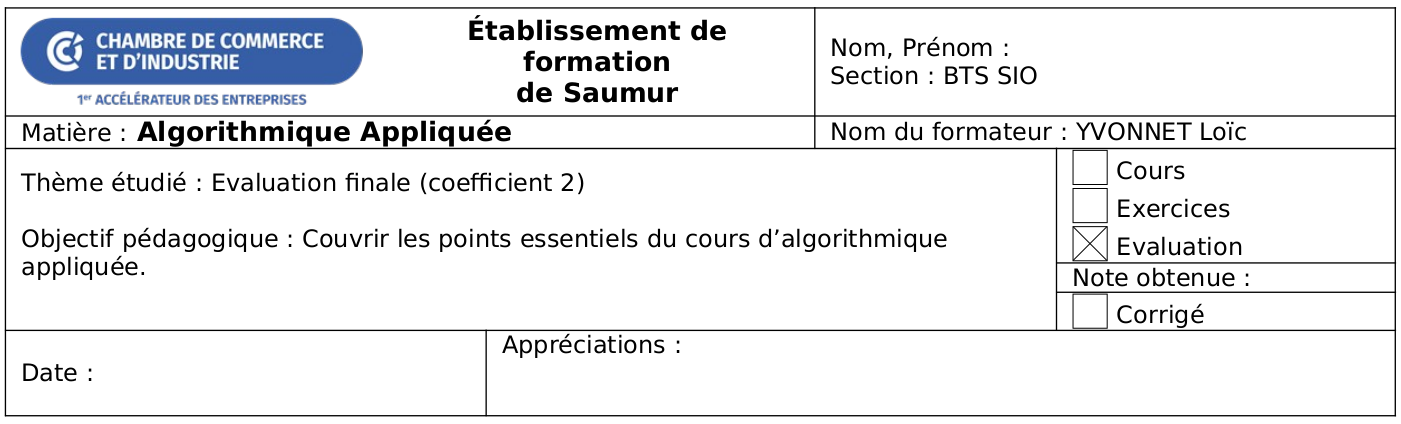
\includegraphics[width=19cm]{assets/entete-cci.png}
\end{figure}

\begin{center}
    Cette évaluation finale donnera lieu à une note sur 20, coefficient 2.

    Vous avez 2h pour répondre aux questions. Vous n'avez pas le droit aux supports de cours, ni ordinateur, ni calculatrice.
\end{center}

\section{Connaissances générales \small{(2 points)}}
\begin{questions}
    \question Que signifie l'expression Turing-complet lorsque l'on parle d'un langage de programmation ?
    \vspace*{1cm}

    \question Qu'est-ce que la dichotomie ? Illustrez avec un exemple.
    \vspace*{3cm}
\end{questions}

\section{Evaluation d'expressions Python \small{(2 points)}}
\begin{questions}
    \question Que valent \texttt{entier} et \texttt{reste} après l'évaluation des expressions Python suivantes ?
    \begin{verbatim}
    entier = 25 // 3
    reste = 25 % 3
    \end{verbatim}
    \vspace*{1cm}

    \question Que vaut \texttt{booleen} après l'évaluation des expressions Python suivantes ?
    \begin{verbatim}
    valeur = 5
    booleen = (valeur == 5)
    \end{verbatim}
    \vspace*{3cm}
\end{questions}

\section{Structures de contrôle \small{(3 points)}}
\begin{questions}
    \question Qu'affiche le programme suivant ? Justifiez votre réponse.
    \begin{verbatim}
    valeur = 5
    if valeur == 10:
        print("beaucoup")
    elif valeur == 5:
        print("un peu")
    else:
        print("pas du tout")
    \end{verbatim}
    \vspace*{1cm}

    \question Qu'affiche le programme suivant ? Justifiez votre réponse.
    \begin{verbatim}
    i = 0
    while i < 3:
        print(i)
        i = i + 1
    \end{verbatim}
    \vspace*{1cm}

    \question Qu'affiche le programme suivant ? Justifiez votre réponse.
    \begin{verbatim}
    chaine = ""
    for i in range(3):
        chaine = chaine + str(i) + " "
    print(chaine)
    \end{verbatim}
    \vspace*{1cm}
\end{questions}

\section{Fonctions \small{(2 points)}}
\begin{questions}
    \question Qu'affiche le programme suivant ? Justifiez votre réponse.
    \begin{verbatim}
    def f(valeur):
        print(valeur)
    
    def g(a, b):
        f(b)
        f(a)
    
    g(5, 3)
    \end{verbatim}
    \vspace*{4cm}

    \question Qu'affiche le programme suivant ? Justifiez votre réponse.
    \begin{verbatim}
    def f(valeur=5):
        return valeur ** 2
    
    def g(fonction, *args):
        resultat = 0
        for valeur in args:
            resultat += fonction(valeur)
    
        resultat += fonction()
    
        return resultat
    
    valeur = g(f, 0, 1, 2)
    print(valeur)
    \end{verbatim}
    \vspace*{1cm}
\end{questions}

\section{Structures de données \small{(2 points)}}
\begin{questions}
    \question Qu'affiche le programme suivant ? Justifiez votre réponse.
    \begin{verbatim}
    liste = [0, 1, 2]
    resultat = []
    for valeur in liste:
        resultat.append(valeur + 1)
    print(resultat[1])
    \end{verbatim}
    \vspace*{1cm}

    \question Qu'affiche le programme suivant ? Justifiez votre réponse.
    \begin{verbatim}
    dico = {"un": 1, "deux": 2}
    dico["trois"] = 3
    for cle, valeur in dico.items():
        print(f"{cle} = {valeur}")
    \end{verbatim}
    \vspace*{1cm}
\end{questions}

\section{Débogage \small{(1 point)}}
\begin{questions}
    \question Décrivez le comportement du code suivant et corrigez-le si nécessaire.
    \begin{verbatim}
    N = int(input("Affichez les entiers positifs jusqu'à : "))
    i = 0
    while i < N:
        print(i + 1)
    \end{verbatim}
    \vspace*{1cm}
\end{questions}

\section{Complexité \small{(2 points)}}
\begin{questions}
    \question Quelle est la complexité de la fonction `f` suivante ? Utilisez la notation Landau $O()$. Justifiez votre réponse.
    \begin{verbatim}
    def f(N):
        compteur = 0
        for i in range(N):
            for j in range(N):
                compteur += 1
        return compteur
    \end{verbatim}
    \vspace*{1cm}

    \question Quelle est la complexité de la fonction `f` suivante ? Utilisez la notation Landau $O()$. Justifiez votre réponse.
    \begin{verbatim}
    def f(a=2, b=3):
        c = a ** 2
        d = b / 3
        e = c + d
        f = e + 3
        g = c * 2 + d * 3 + e + f
        return g + 1
    \end{verbatim}
    \vspace*{1cm}
\end{questions}

\section{Tri \small{(3 points)}}
\begin{questions}
    \question Un jeune enfant possède une collection de cubes. Chacun des cubes comporte une étiquette libellée soit \texttt{"A"}, \texttt{"B"} ou \texttt{"C"}.

    On peut donc représenter la collection de cubes avec une chaîne de caractères telle que : \texttt{"BCAABBCACCBABBC"}.
    
    Ecrivez la fonction \texttt{tri\_cubes} qui prend une chaîne de caractères comportant uniquement des \texttt{"A"}, \texttt{"B"} et \texttt{"C"} et qui renvoie cette chaîne triée.
    
    
    Par exemple :
    \begin{verbatim}
    cubes_dans_l_ordre = tri_cubes("BCAABBCACCBABBC")
    print(cubes_dans_l_ordre)
    \end{verbatim}
    
    doit afficher :
    
    \begin{verbatim}
    AAAABBBBBBCCCCC
    \end{verbatim}
    
    \vspace*{5cm}

\end{questions}

\section{Addition de matrices \small{(3 points)}}
\begin{questions}
    \question On utilise une \texttt{list} de \texttt{list} pour représenter une matrice.

    Par exemple, la matrice $M$ :

    $$
    M =
    \begin{pmatrix}
        1 & 2 \\
        3 & 4
    \end{pmatrix}
    $$

    est représentée de la manière suivante :

    \begin{verbatim}
    M = [
        [1, 2],
        [3, 4]
    ]
    \end{verbatim}

    Ecrivez la fonction \texttt{additionne\_matrices} qui prend 2 matrices en entrée et renvoie leur somme.

    Pour rappel :

    $$
    M =
    \begin{pmatrix}
        a & b \\
        c & d
    \end{pmatrix}
    ,\quad
    N =
    \begin{pmatrix}
        e & f \\
        g & h
    \end{pmatrix}
    $$
    $$
    S = M + N =
    \begin{pmatrix}
        a + e & b + f \\
        c + g & d + h
    \end{pmatrix}
    $$

    Par exemple :
    \begin{verbatim}
    M = [
        [1, 2],
        [3, 4]
    ]
    print(f"M = {M}")

    N = [
        [1, 0],
        [0, 1]
    ]
    print(f"N = {N}")

    S = additionne_matrices(M, N)
    print(f"S = {S}")
    \end{verbatim}

    doit afficher :
    \begin{verbatim}
    M = [[1, 2], [3, 4]]
    N = [[1, 0], [0, 1]]
    S = [[2, 2], [3, 5]]
    \end{verbatim}   
    \vspace*{5cm}
\end{questions}

\end{document}